\chapter{Motivation}
\label{motivation}

The goal of this thesis is to create a network that can be analyzed in the hope of understanding the causes of side effects for any drug represented in the network. The assumption is that a relationship triangle can be created in which chemicals, targets and phenotypes are associated with each other, see Figure ~\ref{fig:workflow}.1. In which case, the cause of side effects can be understood by analyzing the mechanism of action of drugs.

To achieve the goals of the project first, a knowledge graph is created. This graph contains three different types of entities: chemicals, targets, and phenotypes; and three different relations, chemical-chemical, chemical-target and chemical-phenotype. Then, different \ac{NRL} approaches are used to create embeddings of the graph, which are then trained and optimized to obtain the best model. This model is then used to predict new relations with different node types, which are then analyzed using literature. A schematic of the workflow is presented in Figure ~\ref{fig:workflow}.

\begin{figure}[!ht]
    \centering
    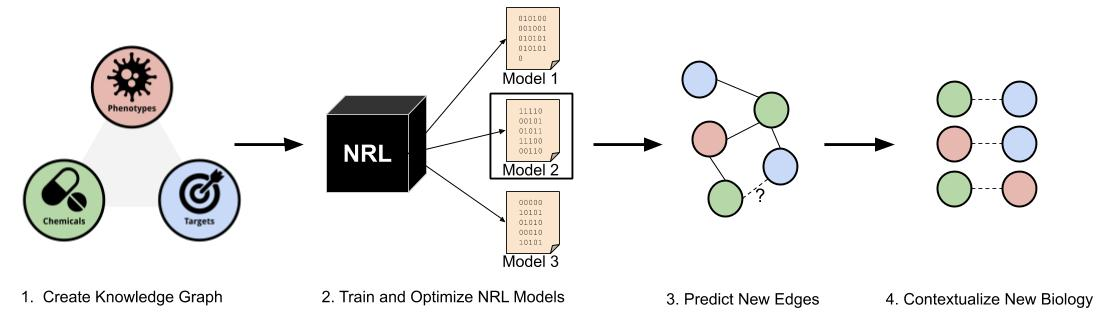
\includegraphics[scale=0.35]
    {figures/workflow.jpg}
    \caption [The workflow of the project]{\label{fig:workflow} The workflow of the project. 1. Create knowledge graph that contains chemicals, targets and phenotypes. 2. Train different NRL models and optimize them. 3. Use the best NRL model to predict new edges. 4. Contextualize the new knowledge.}
\end{figure}